\documentclass[a4paper,12pt]{article}
\parindent 0pt
\parskip 1mm
\usepackage[dvips]{epsfig}

\begin{document}

\begin{center}
{\Large\bf CN 510 - Principles and Methods of Cognitive and Neural Modeling}

\bigskip

{\large\bf Assignment \# 1}
\smallskip

{\large\bf John Joseph}
\end{center}

We are given the following non-homogeneous differential equation

\begin{equation}
\frac{dx}{dt} + Ax = I
\end{equation}

\bigskip
{\bf Analytic Solution}
\bigskip

The solution of course exists in two parts: homogeneous, and particlar. The homogenous solution can be found as follows:

\begin{equation}
\frac{dx_h}{dt} + Ax_h = 0
\end{equation}
\begin{equation}
\frac{dx_h}{dt} = -Ax_h
\end{equation}
\begin{equation}
x_h(t) = Ce^{-At}
\end{equation} 

Now that we have the homogeneous solution, let us solve for the particular solution. 

\begin{equation}
\frac{dx_p}{dt} + Ax_p = I
\end{equation}
\begin{equation}
x_p(t) = mt+b
\end{equation}
\begin{equation}
\frac{dx_p}{dt} + Ax_p = m + A(mt+b) = I
\end{equation}
\begin{equation}
m = 0
\end{equation}
\begin{equation}
b = \frac{I}{A}
\end{equation}
\begin{equation}
x_p(t) = \frac{I}{A}
\end{equation}

Adding together the homogeneous and particular solution, we get

\begin{equation}
x(t) = Ce^{-At} + \frac{I}{A}
\end{equation}

To solve for the constant C, we must rely on an initial state of our system; let us say that when $t=0$, $x(0)=x_0$.

\begin{equation}
x(0) = x_0 = C + \frac{I}{A}
\end{equation}

\begin{equation}
C = x_0 - \frac{I}{A}
\end{equation}

Thus, the solution to the differential equation is 

\begin{equation}
x(t) = (x_0 - \frac{I}{A})e^{-At} + \frac{I}{A}
\end{equation}

As you can see, this equation depends on three initial parameters: $x_0$, $I$, and $A$. These will be required not only to fully solve and plot the analyitic solution; we also require these boundary conditions be set in order to use numerical methods in calculating the solution.

{\bf Analytic Results}
\bigskip 

Note that the system described by the equation 

\begin{equation}
x(t) = (x_0 - \frac{I}{A})e^{-At} + \frac{I}{A}
\end{equation}

actually converges to an equilibrium state as our variable representing time, $t$, approaches larger values. We can see the exponential portion of the term contains a negative sign in its power, so as $t$ gets larger and larger the exponential term starts to vanish. 

\vspace{2mm}

Once this term has grown sufficiently small, the outcome of the above equation will be extremely close to the constant term $\frac{I}{A}$. This is the equilibrium solution as $t\rightarrow\infty$. 

\begin{eqnarray}
A=1, I=5,  x\rightarrow\frac{I}{A}=5 \\
A=1, I=0,  x\rightarrow\frac{I}{A}=0 \\
A=2, I=5,  x\rightarrow\frac{I}{A}=2.5 \\
A=1, I=5,  x\rightarrow\frac{I}{A}=0
\label{array1}
\end{eqnarray}

\begin{figure}[!ht]
\begin{center}
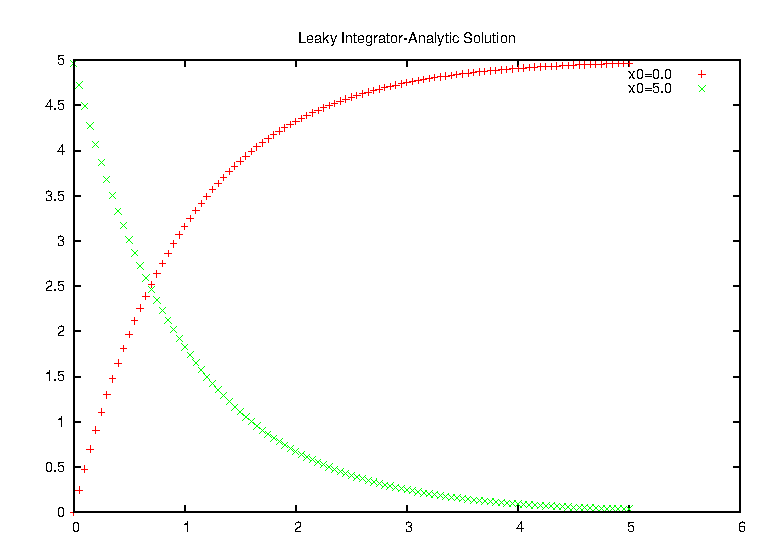
\epsfig{file=data/figures/a_1_2,width=13cm,height=10cm}
\end{center}
\caption{\label{pict1} Two initial conditions: $A=1,I=5,x_0=0$ and $A=1,I=0,x_0\approx5$}
\end{figure} 

From the plot above we can see that our results approach these equilibrium states, states which again depend on the initial conditions. For example, when $x_0=0.0$, $I=5$ and $A=1$, we see the solution eventually converges on $x=5.0$. Similarly, when $x_0=5.0$ and $I=0$, the results will inevitable converge on $x=0.0$ as $t\rightarrow5$. 

\vspace{2mm}

This trend can be seen again in the plots for the other two initial conditions, which are shown at the end of the document. 

\vfil\eject

{\bf Numerical Results}
\bigskip 

Now that we have plotted the analytical solution to the Leaky Integrator, we turn to numerical integration methods to see how they hold up against the real thing. The three methods used were Rotter-Deismann, Euler, and Runge-Kutta.

\begin{figure}[h!]
\begin{center}
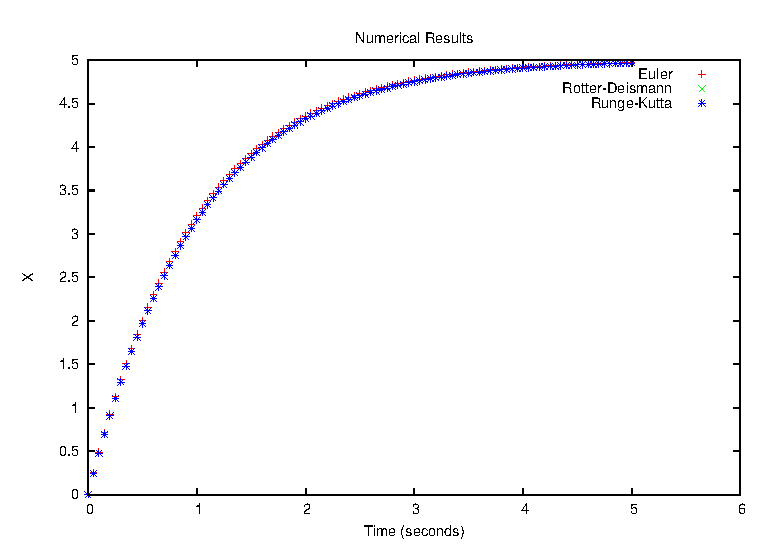
\epsfig{file=data/figures/n_1,width=13cm,height=10cm}
\end{center}
\caption{\label{pict2} The numerical results to the three simulation methods discussed above for I=5,A=1,x0=0. }
\end{figure}

Looking at the above plots, it may be difficult to see which integration method is the best. It can also be difficult at times to discern between the different methods, so I have plotted here the differences between the analytic solution and these three numerical methods. 

\vfil\eject

Surprisingly, the Rotter-Deismann and Runge-Kutta methods were equal to the analytic solution {\bf down to the last digit}. I did not believe this at first, so I ran some tests using double precision and a smaller time step in the numerical methods only. 

I found that,for example, the Analytic solution yielded a number like 0.47581290, while the Rotter-Deismann method yielded a number like 0.47581246. These two numbers have a difference of 0.00000044, which borders on the lowest possible values capable of being understood by my computer. 

\begin{figure}[h!]
\begin{center}
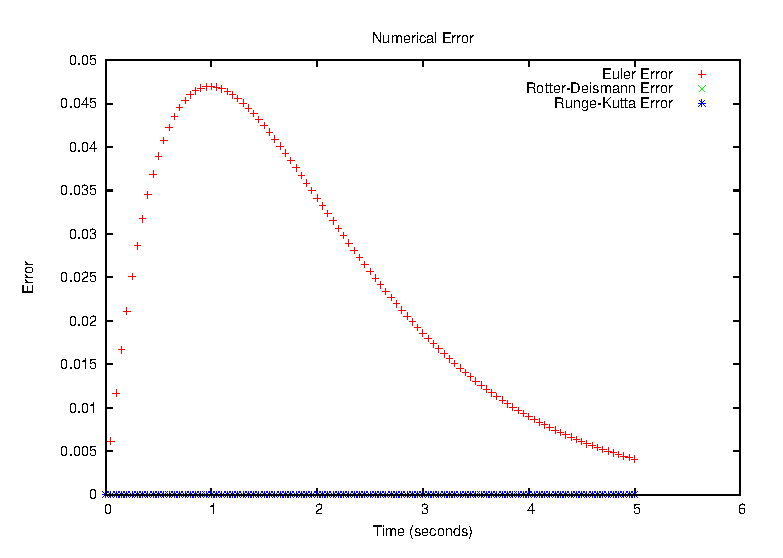
\epsfig{file=data/figures/n_e_1,width=13cm,height=10cm}
\end{center}
\caption{\label{pict3} The numerical error of these three integration methods. }
\end{figure}

As you can see, the Rotter-Deismann and Runge-Kutta errors are zero. The Euler error is a bit more interesting; we can see that for values of $t<1$ the error grows, but once $t>1$ the error quickly converges toward zero. 

\vfil\eject

{\bf Conclusions}
\bigskip

For this very simple example we can see that some well known numerical methods are extremely capable of producing accurate results. We should not expect this for more complex systems, but the assignment was a good exercise in analysis. 

\vspace{2mm}

The effect of A on the system brings to mind two things. The first is the equilibrium solution, $\frac{I}{A}$, and the second is the exponential term $Ce^{-At}$. The equilibrium solution is inversely proportional to A, and the rate of convergence (that is, how fast the exponential term drops to 0) is directly proportional to A. Thus, larger values of A lead to lower equilibrium values, and the system will reach these values at an increased rate. 

\vspace{2mm}

Attached at the end of this report are the analytic plots of the remaining two situations. The promise of extra credit incited me to perform the simulation using both 32 bit and 64 bit floating point values, which is easily done in C by using the typedef construct. 

\vspace{2mm}

The data for these two types of simulations will be included (as text files) with this report, along with the C source code used to generate them. I understand that this code was to be put directly in this document, but it took up an exorbitant amount of space. I hope this is not a problem. 

\vfil\eject

\begin{figure}[h!]
\begin{center}
\epsfig{file=data/figures/a_3_4,width=13cm,height=8cm}
\end{center}
\caption{\label{pict4}Two initial conditions: $A=2,I=5,x_0=0$ and $A=2,I=0,x_0\approx2.5$}
\end{figure}

\begin{figure}[h!]
\begin{center}
\epsfig{file=data/figures/4_all,width=13cm,height=8cm}
\end{center}
\caption{\label{pict5}Overlay of all results for the above conditions}
\end{figure}


\end{document}
